\subsubsection{Mechanism for scoring autonomous climbers and pushing button}
\paragraph{Plan of creating module:}	
	
	\begin{enumerate}
		\item Creating 3D model in Creo parametric.
		\item Calculation of moments, distances and angels.
		\item Testing and debugging of the mechanism
	\end{enumerate}
	
	The module turns F-shaped beam using servo. On the top of beam is a bucket with climbers. After beam turns, bucket turns over. Climbers go to the box. At the end of other part of a beam is a light sensor. He detects color of a button and presses it. Robot performs it at autonomous period.
  \begin{figure}[H]
		\begin{minipage}[h]{\linewidth}
			\center{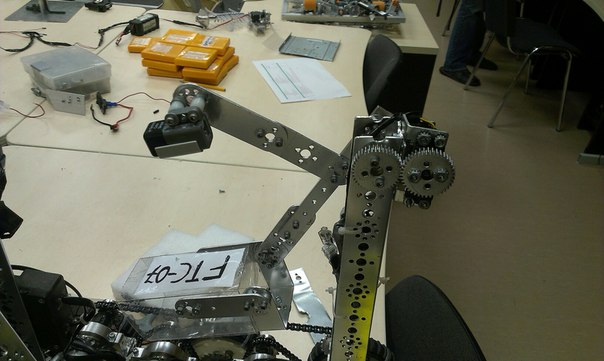
\includegraphics[scale=0.5]{days_L/Meetings/images/08}}
			\caption{F-beam module}
		\end{minipage}
	\end{figure}
	
	\paragraph{Ideas that were looked:}
	
	\begin{enumerate}	
		\item The first idea was the following: we decided to use two beams. Two beams turns, the light sensor on the end of each beam detects the correct button. Beam, which detects the correct button wrests in place. The other beam turns up. The robot goes forward and presses the correct button. But this idea isn't good because we using two servos and this is very difficult and the module take up much up space.
	
		\item Another idea was the following: we decided to use one beam. The beam turns and the light sensor on the end of the beam detects the color of the right button. If this color is correct, the robot turns right and then goes forward. Else the robot turns left and then goes forward. This algoritm is slower, but it's lighter and the model takes not as much space. We decided to use twice algoritm.
	\end{enumerate}
	
	\paragraph{Calculation of moments}
	
	We calculated the moments to compare it with the maximum moment of the servo. If the maximum moment of the servo is higher than the moment of module, the module will work. The maximum moment of the servo(HS-485HB) is 28 kg*mm. The moment of gravity forces using the following formulae: 
	
	$m_\text{constr} \cdot l_\text{constr} + m_\text{climbers} \cdot l_\text{climbers}$.	
	 $M_\text{constr}$ is the total mass of the module without climbers. $L_\text{constr}$ is the distance between the rotation axis and the COG of module without climber. $M_\text{climbers}$ is the total mass of the two climbers. $L_\text{climbers}$ is the distance between the rotation axis and the COG of climbers. All values we find in Creo Parametric.
	 
	 $M_\text{constr}$ is about 100 g or 0.1 kg. $L_\text{constr}$ is about 93 mm. The moment of construction is about 9.3 kg*mm. Mass of a climber is 22.7 g. Mass of two climbers is 0.0454 kg. The COG of climbers and geometrical center ar ine the same place, because the climbers are uniform. It is about 204 mm. The moment of gravity forces if the all module is 18.9 kg*mm. Safety factor is 1.5. With this factor moment of module is 28 kg*mm. The moment of module is not bigger than the maximum moment of the servo. The module will work.
	 %\begin{figure}[H]
	 %	\begin{minipage}[h]{\linewidth}
	 %		\center{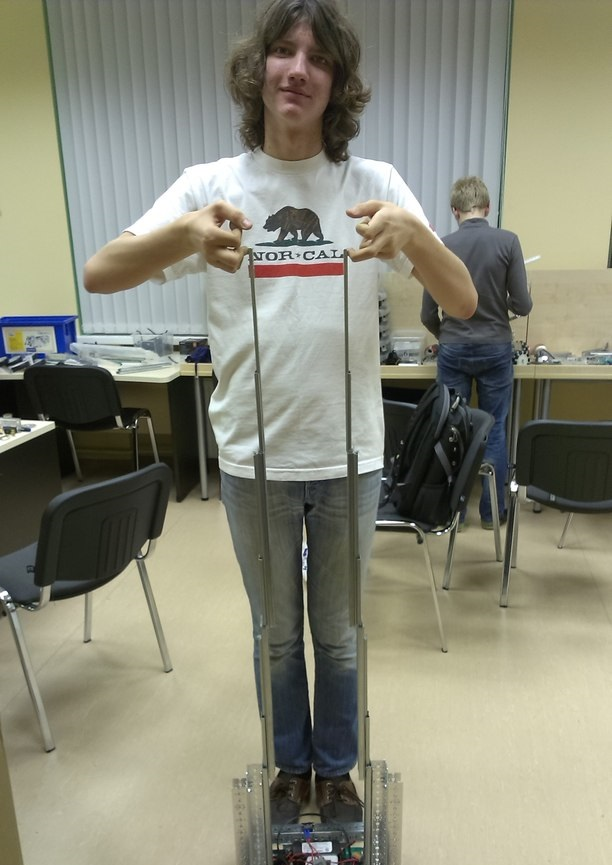
\includegraphics[scale=0.7]{days_L/f-beam/images/02}}
	 %		\caption{The table of moments}
	 %	\end{minipage}
	 %\end{figure}
	 
	 \paragraph{Work of module}
	 
	 \begin{itemize}
	 
		 \item A dimension of the bucket is 6x5.5x12 mm. A dimenension of the main beam is 20x0.5x1.5 mm.
	 
		 \item The robot must stay near the button on the distance 16.9 cm. Also the main beam must be in the middle of the beacon. Than the robot turns beam on 48 degrees and the climbers go down. Than the robot must go forward on the distance 5 cm. After that the robot turns beam on 42 degrees. Than the robot detects correct button and turns in his side on 9 degrees. At the end the robot goes forward and presses correct button.
	\end{itemize}
	\fillpage
